\documentclass[11pt]{amsbook}

\usepackage{../HBSuerDemir}


\begin{document}

% ++++++++++++++++++++++++++++++++++++++
\hPage{b1p2/385}
% ++++++++++++++++++++++++++++++++++++++
bounded by y = f(x), the tangent line at P and the vertical lines x = a,x = b be an extremum.

\begin{enumerate}

\item[81.]
If $a<b<c$, show that the area bounded by the curves of y = $(x-2a)^2$, y = $(x-2b)^2$ and y = $(x-2c)^2$ is equal to 2(c-a)(c-b)(b-a).
\item[82.]
Find the area under the curve of f(x)$\geq$ 0 over the given interval:

\begin{tabular}{ll}
a)f(x) = $x\sqrt{2x^2+1}, (0, 2)$
&b)f(x) = $\frac{sin 2x}{cos^2 2x}$ , (0, $\pi$/6)
\end{tabular}

\item[83.]
Find a relation for $\lambda$ such that the vertical segment (P0) bisects the shaded area under the quarter of unit circle.

\begin{figure}[htb]
\begin{center}
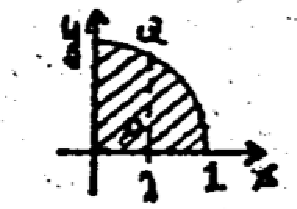
\includegraphics[width=0.20\textwidth]{images/b1p2-385-fig01}
\end{center}
\end{figure}

\item[84.]
Find the area of the region bounded by the curve y = $x^3$ - $6x^2$, the tangent line at its inflection point and the lines x=0, x=6.
\item[85.]
Given the parabola y = $x^2$ and a point P = (t, $t^2$) on it, find t\textgreater0 such that the area between the parabola and the normal line at P be minimum.

\item[86.]
The curve is a quarter of an ellipse.Determine $\tan\theta$ 
for which the shaded areas be equal to each other.

\begin{figure}[htb]
\begin{center}
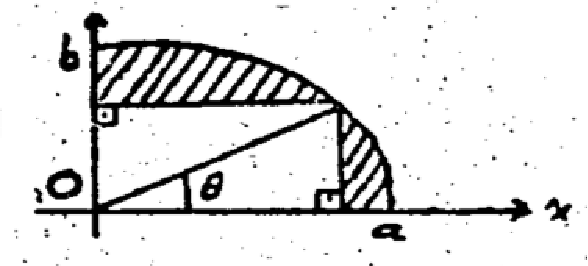
\includegraphics[width=0.20\textwidth]{images/b1p2-385-fig02}
\end{center}
\end{figure}

\item[87.]
Compute the area of the region enclosed by the curve of
y = $(x^3-8)/x^2$, and its tangent line at x = 2 and the joining
the points (-2, -4), (2, 0).
\item[88.]
Compute the area of the region defined by y - $x^3$ \textgreater 0, $y^2$ - 32x \textless 0 and 6x + y - 7 \textgreater 0.
\item[89.]
Compute the area of the region bounded by

\begin{tabular}{ll}
a) y = (x-1)/$x^3$, x=20, x-axis 
&b) y = 1/$\sqrt{x+3}$, x=0, x=1, x=6\\
c) y = x/$\sqrt{x^2+9}$, y=0, x=4
\end{tabular}
\end{enumerate}
\end{document}